%%%%%%%%%%%%%%%%%%%%%%%%%%%%%%%%%%%%%%%%%%%
%% ---
%\chapter{Resposta ao pedido de obtenção dos bancos de dados}\label{chap:esic}
%%% ---
%
%Prezado(a) Sr(a) Haydée Svab
%
%CONFIRMAMOS O RECEBIMENTO DE SUA SOLICITAÇÃO de acesso a documentos, dados e informações.
%
%Anote o número do seu protocolo: 58206146035
%
%Data: 05/05/2014
%
%Órgão/Entidade:  Companhia do Metropolitano de São Paulo
%
%SIC:  Companhia do Metropolitano de São Paulo – METRÔ
%
%Forma do recebimento da resposta: Buscar/Consultar pessoalmente
%
%Solicitação:
%Sou mestranda do programa de Engenharia de Transportes da Escola Politécnica da Universidade de São Paulo e solicito a disponibilização e liberação das bases de dados (microdados) das Pesquisas Domiciliares de Origem e Destino de 1977, 1987 e 2002 para fins acadêmicos, podendo ser utilizadas como fonte de trabalhos e artigos.
%Envio anexa carta do meu orientador, Prof. Dr. Orlando Strambi, ratificando o pedido.
%Grata pela atenção,
%Haydée Svab
%
%A sua solicitação será atendida no PRAZO não superior a 20 (vinte) dias, a contar da data do protocolo da solicitação, de acordo com o \S1º do artigo 15 do Decreto nº 58.052, de 16/05/2012.
%
%O prazo referido acima poderá ser prorrogado por mais 10 (dez) dias, mediante justificativa expressa, da qual será cientificado o interessado, conforme o \S2º do mesmo artigo.
%
%Dentro deste prazo o interessado será informado, também, sobre a data, local e modo para se realizar a consulta, efetuar a reprodução ou obter a certidão, ou sobre as razões de fato ou de direito da recusa, total ou parcial, do acesso pretendido.
%
%Atenciosamente,
%
%SIC.SP - Governo do Estado de São Paulo 
%%%
%%%%%%%%%%%%%%%%%%%%%%%%%%%%%%%%%%%%%%%%%%%
%% ---
\chapter{Correspondência entre Zonas das Pesquisas Origem Destino por meio das Unidades de Correspondência entre Zonas (UCOD)}\label{chap:anexo_ucod}
%% ---
\includepdf{anexos/UCOD01.pdf}
\includepdf{anexos/UCOD02.pdf}
\includepdf{anexos/UCOD03.pdf}
%% ---
%%%%%%%%%%%%%%%%%%%%%%%%%%%%%%%%%%%%%%%%%%%
%% ---
\chapter{Mapas de Zonas e Subzonas das Pesquisas Origem Destino (1977, 1987, 1997 e 2007)}\label{chap:anexo_mapas_zonas}
%% ---
%\includepdf{anexos/Mapa-zonas1977.pdf}
%\includepdf{anexos/Mapa-zonas1987.pdf}
%\includepdf{anexos/Mapa-zonas1997.pdf}
%\includepdf{anexos/Mapa-zonas2007.pdf}
%% ---
%%%%%%%%%%%%%%%%%%%%%%%%%%%%%%%%%%%%%%%%%%%
%% ---
\chapter{Layouts dos bancos de dados das Pesquisas Origem-Destino do Metrô-SP (1977, 1987, 1997 e 2007)}\label{chap:anexo_layouts}
%% ---
\includepdf[pages=-]{anexos/layout77.pdf}
\includepdf[pages=-]{anexos/layout87.pdf}
\includepdf[pages=-]{anexos/layout97.pdf}
\includepdf[pages=-]{anexos/layout07.pdf}
%% ---
%%%%%%%%%%%%%%%%%%%%%%%%%%%%%%%%%%%%%%%%%%%
%% ---
\chapter{Rotinas de Preparação das Bases de Dados das Pesquisas Origem-Destino do Metrô-SP (1977, 1987, 1997 e 2007)}\label{chap:anexo_rotinas}
%% ---
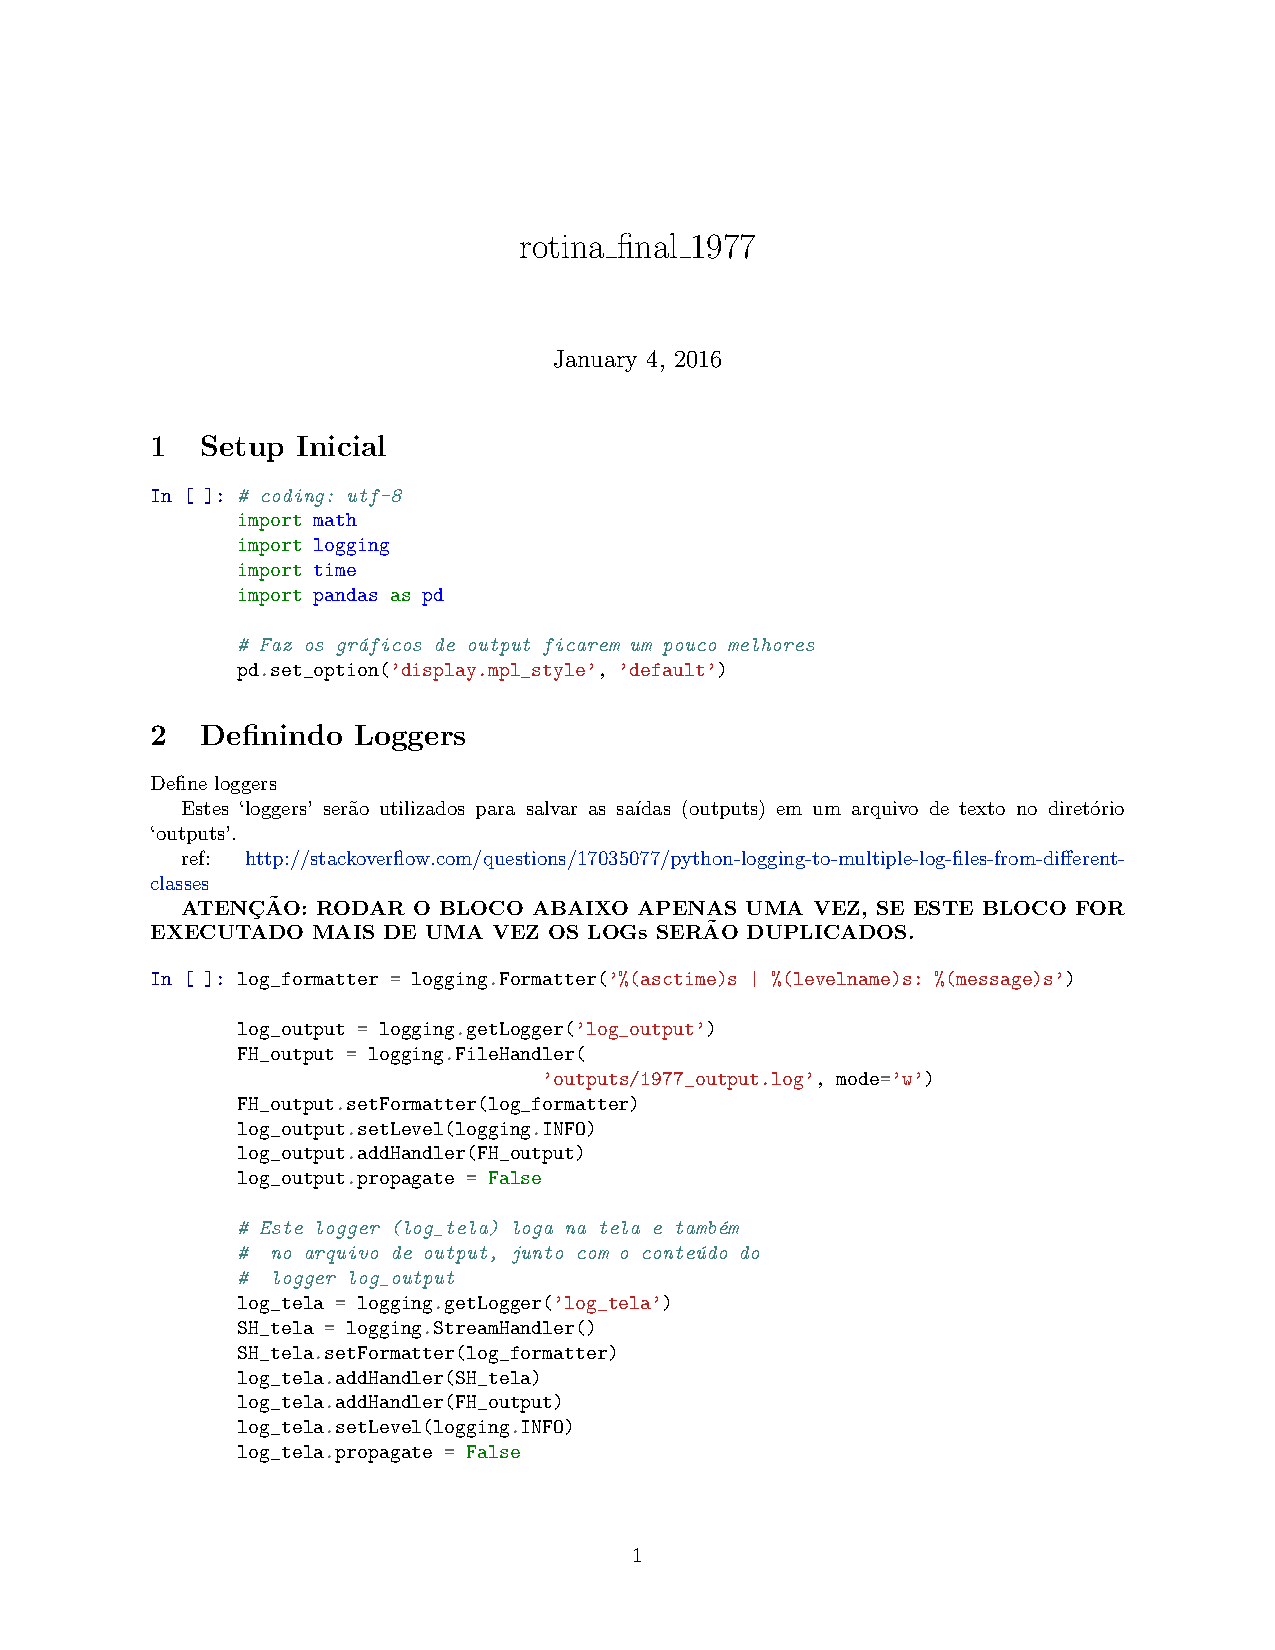
\includepdf[pages=-]{anexos/rotinafinal1977.pdf}
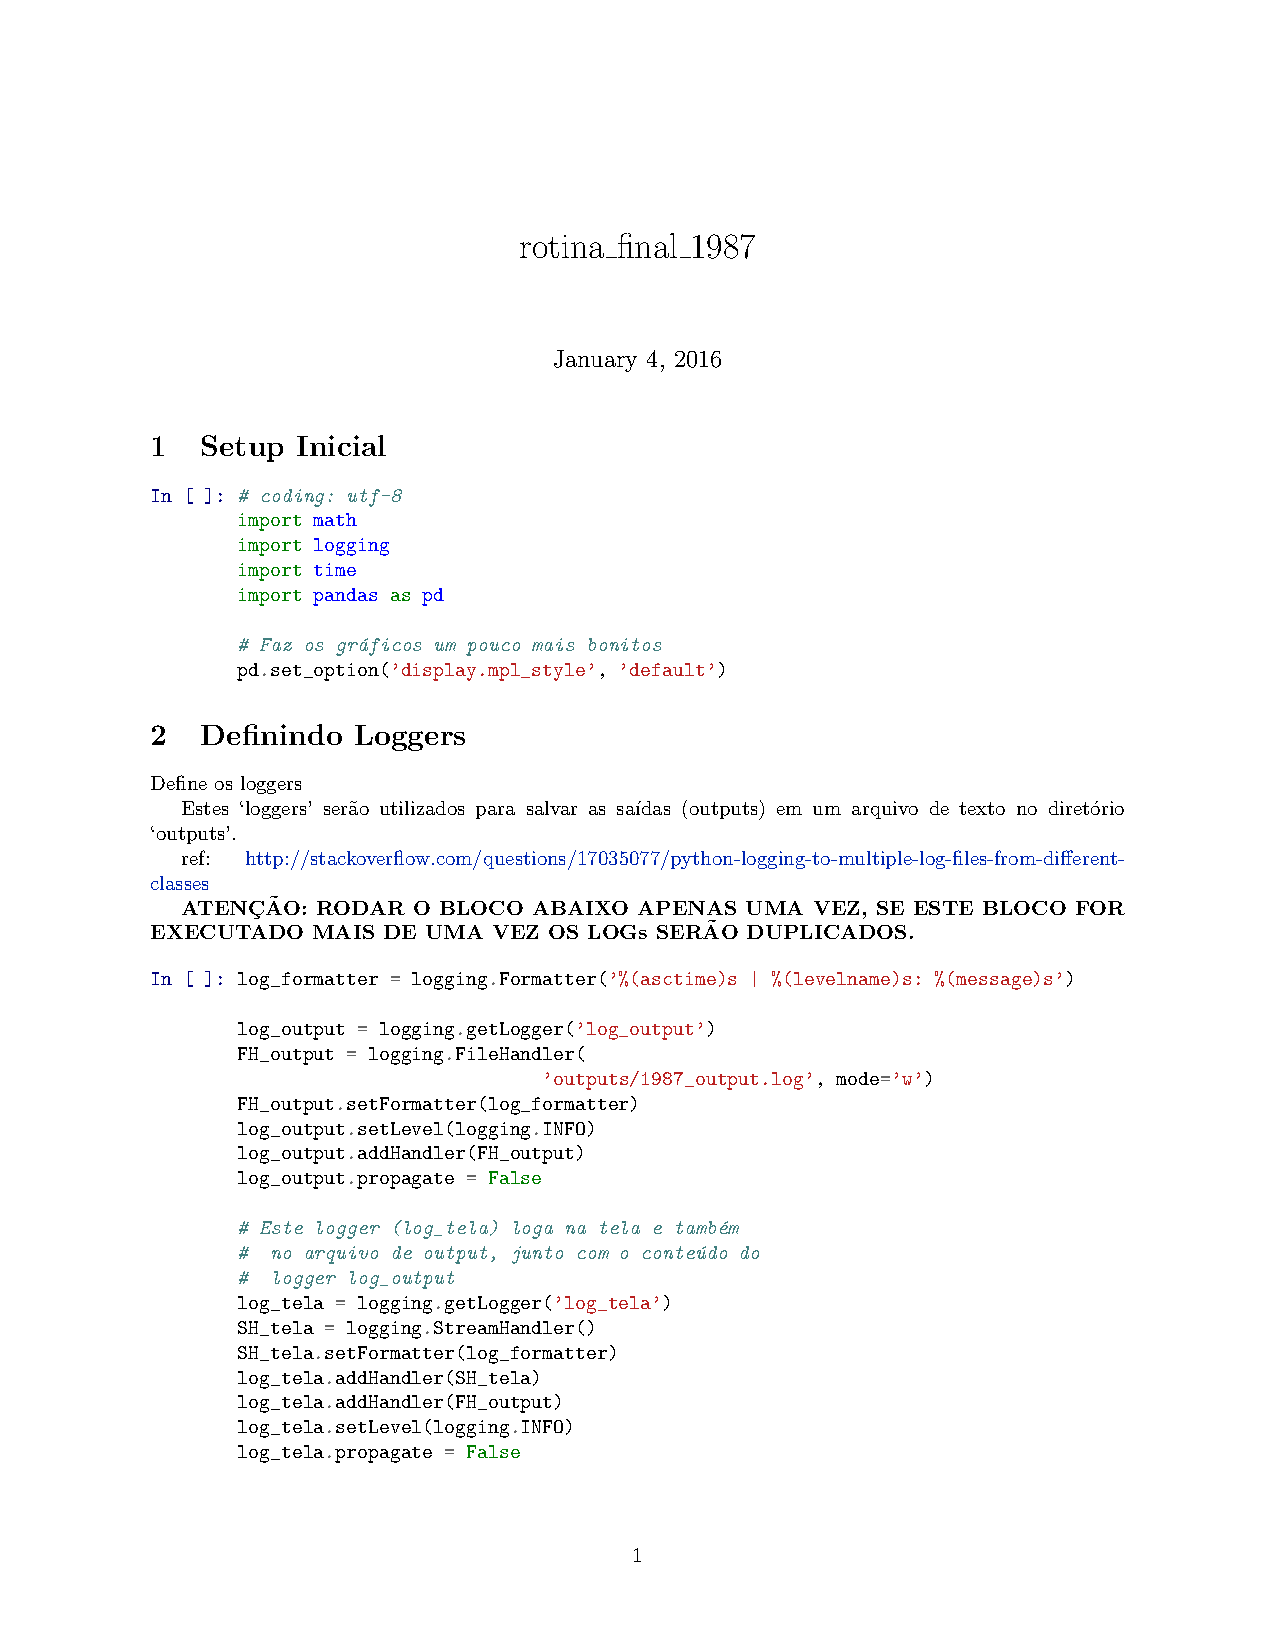
\includepdf[pages=-]{anexos/rotinafinal1987.pdf}
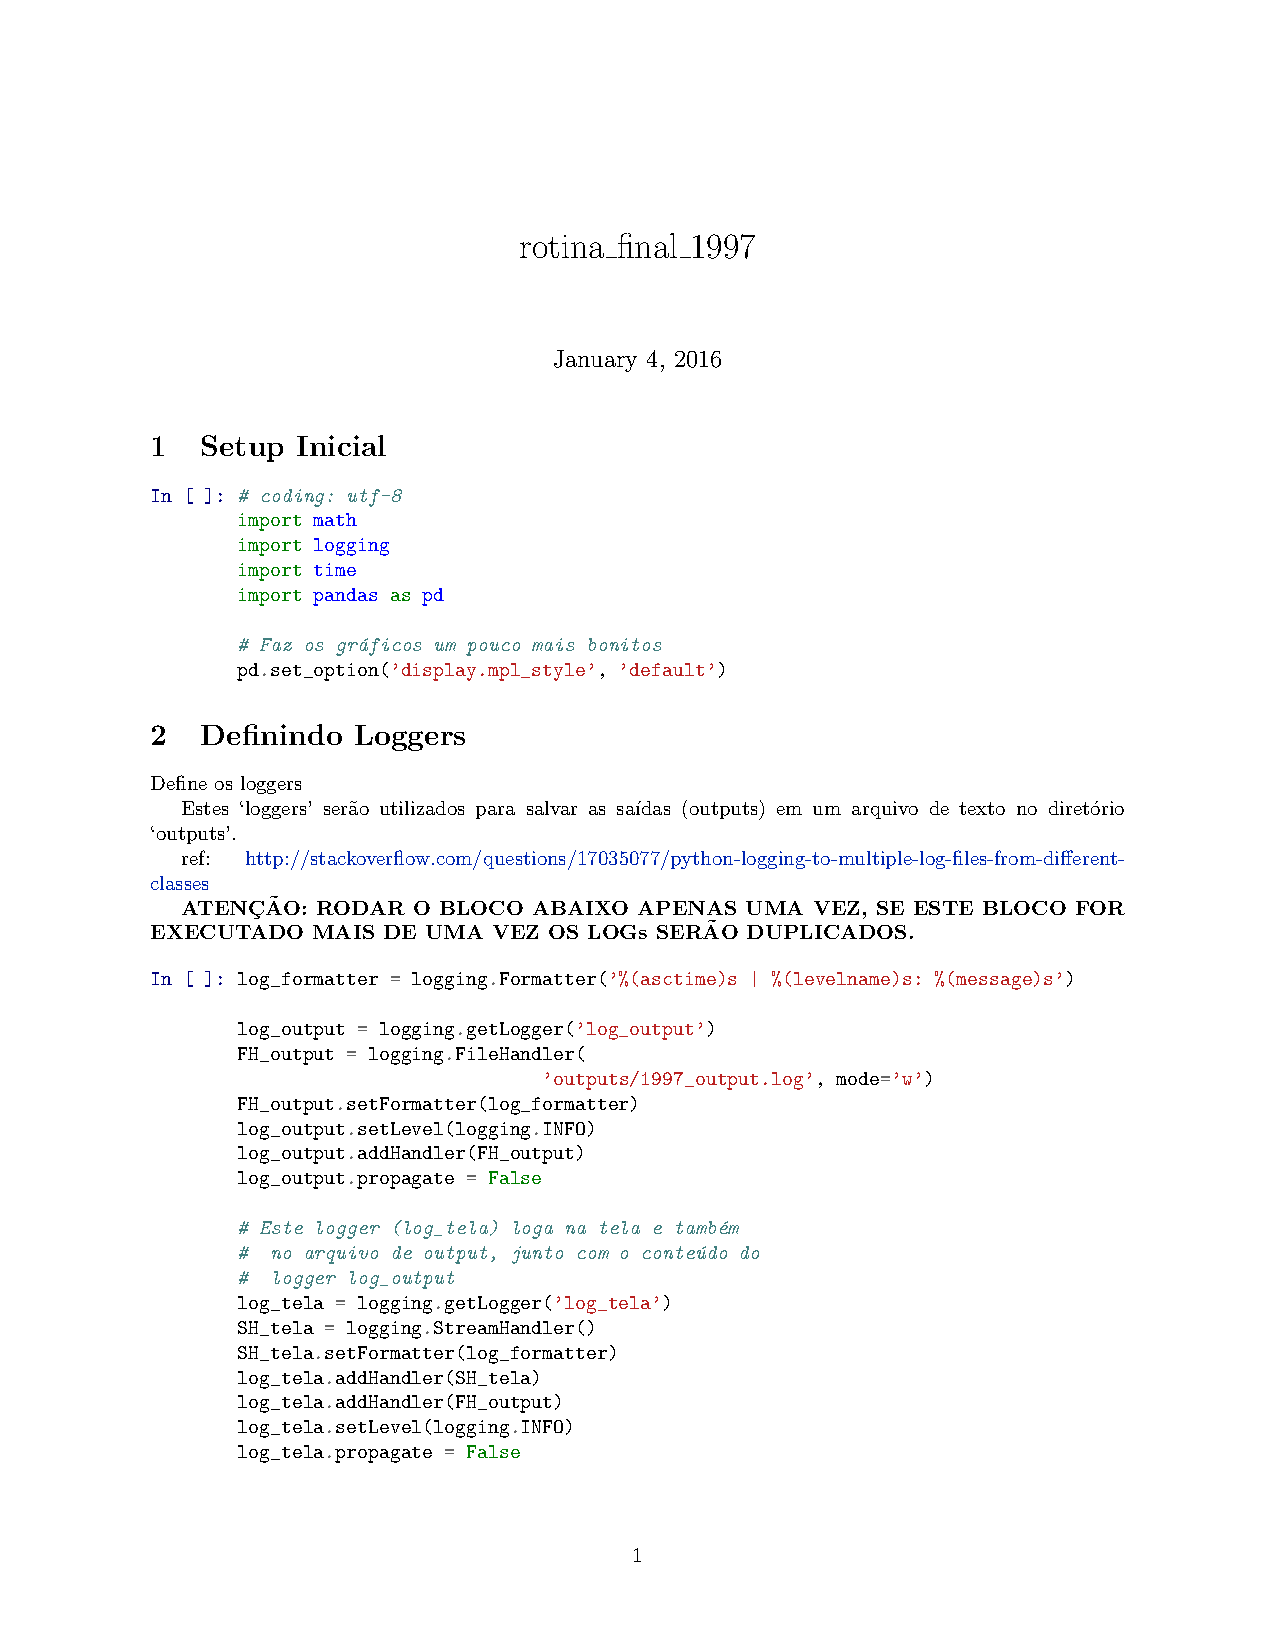
\includepdf[pages=-]{anexos/rotinafinal1997.pdf}
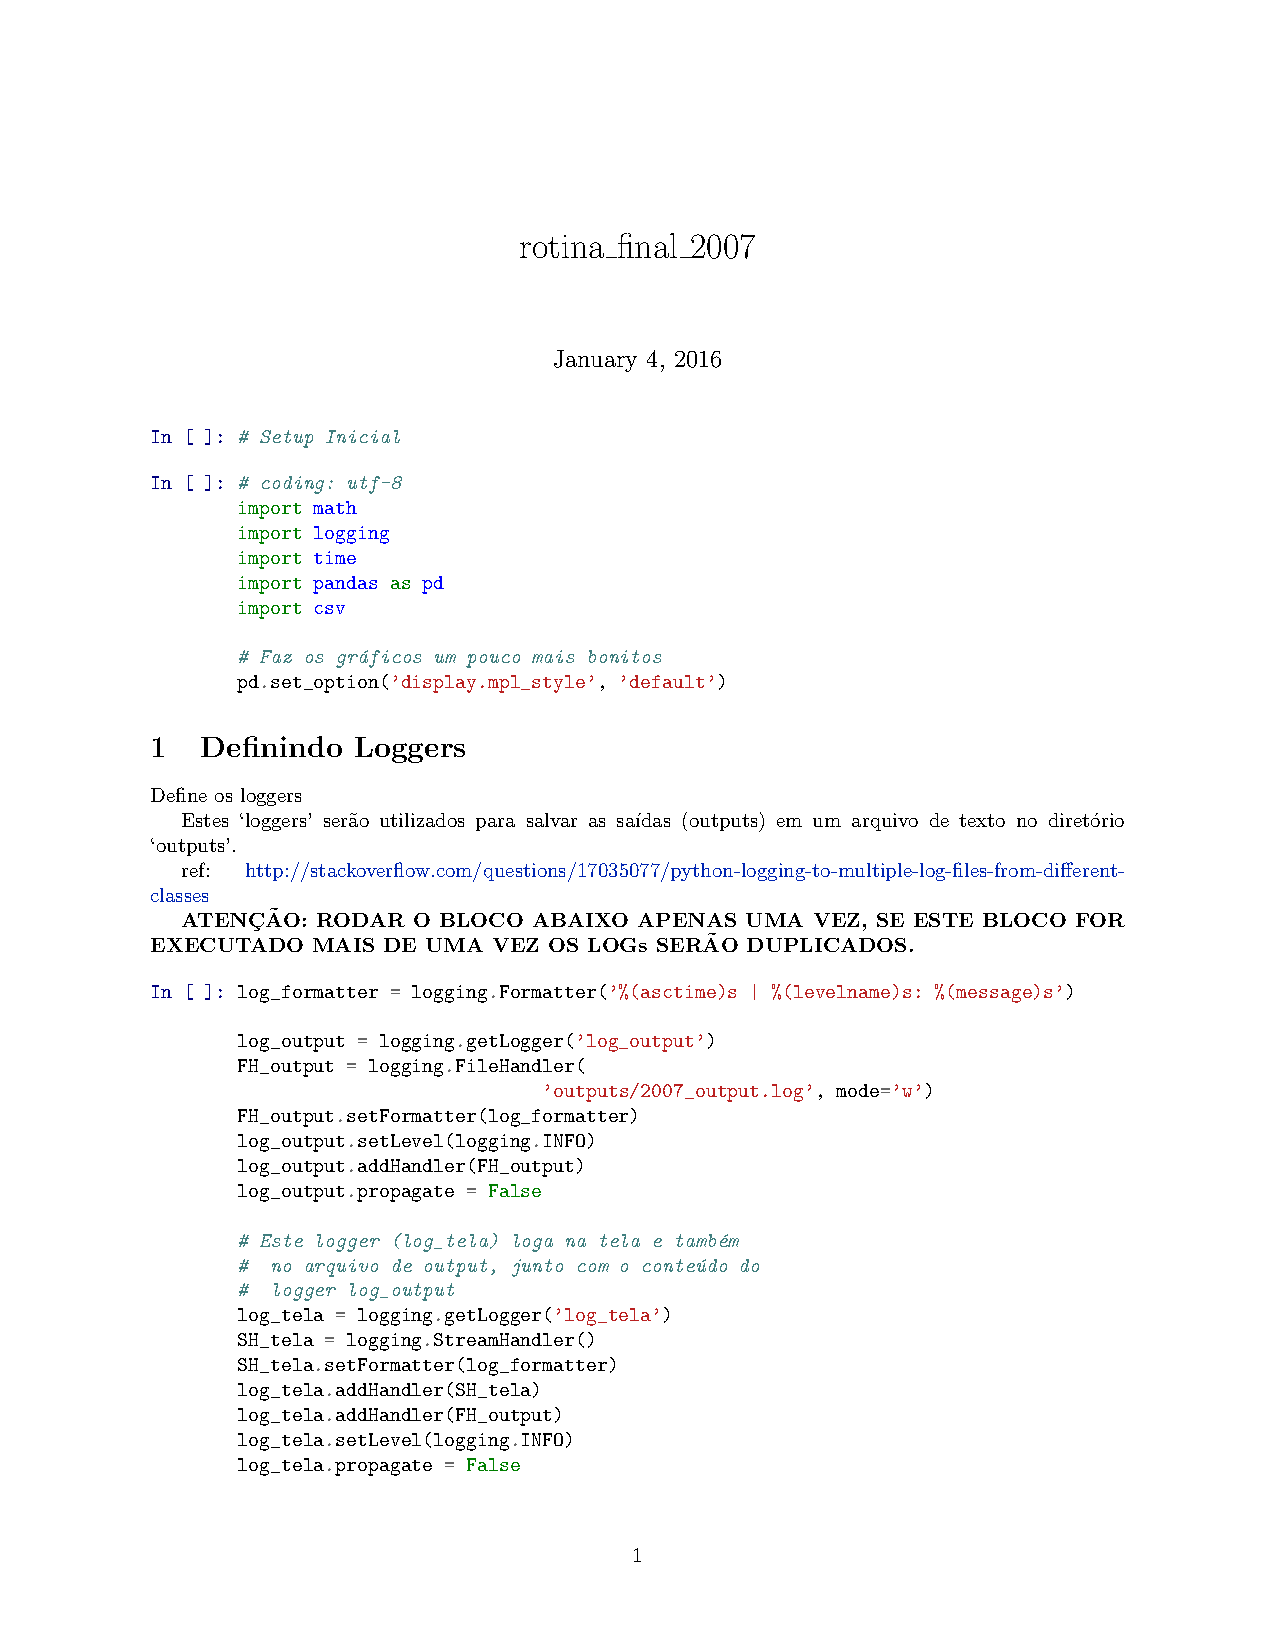
\includepdf[pages=-]{anexos/rotinafinal2007.pdf}
%% ---
%%%%%%%%%%%%%%%%%%%%%%%%%%%%%%%%%%%%%%%%%%%
%% ---
\chapter{Síntese de resultados para 4 conglomerados}\label{chap:anexo_4_clusters_td}
%% ---
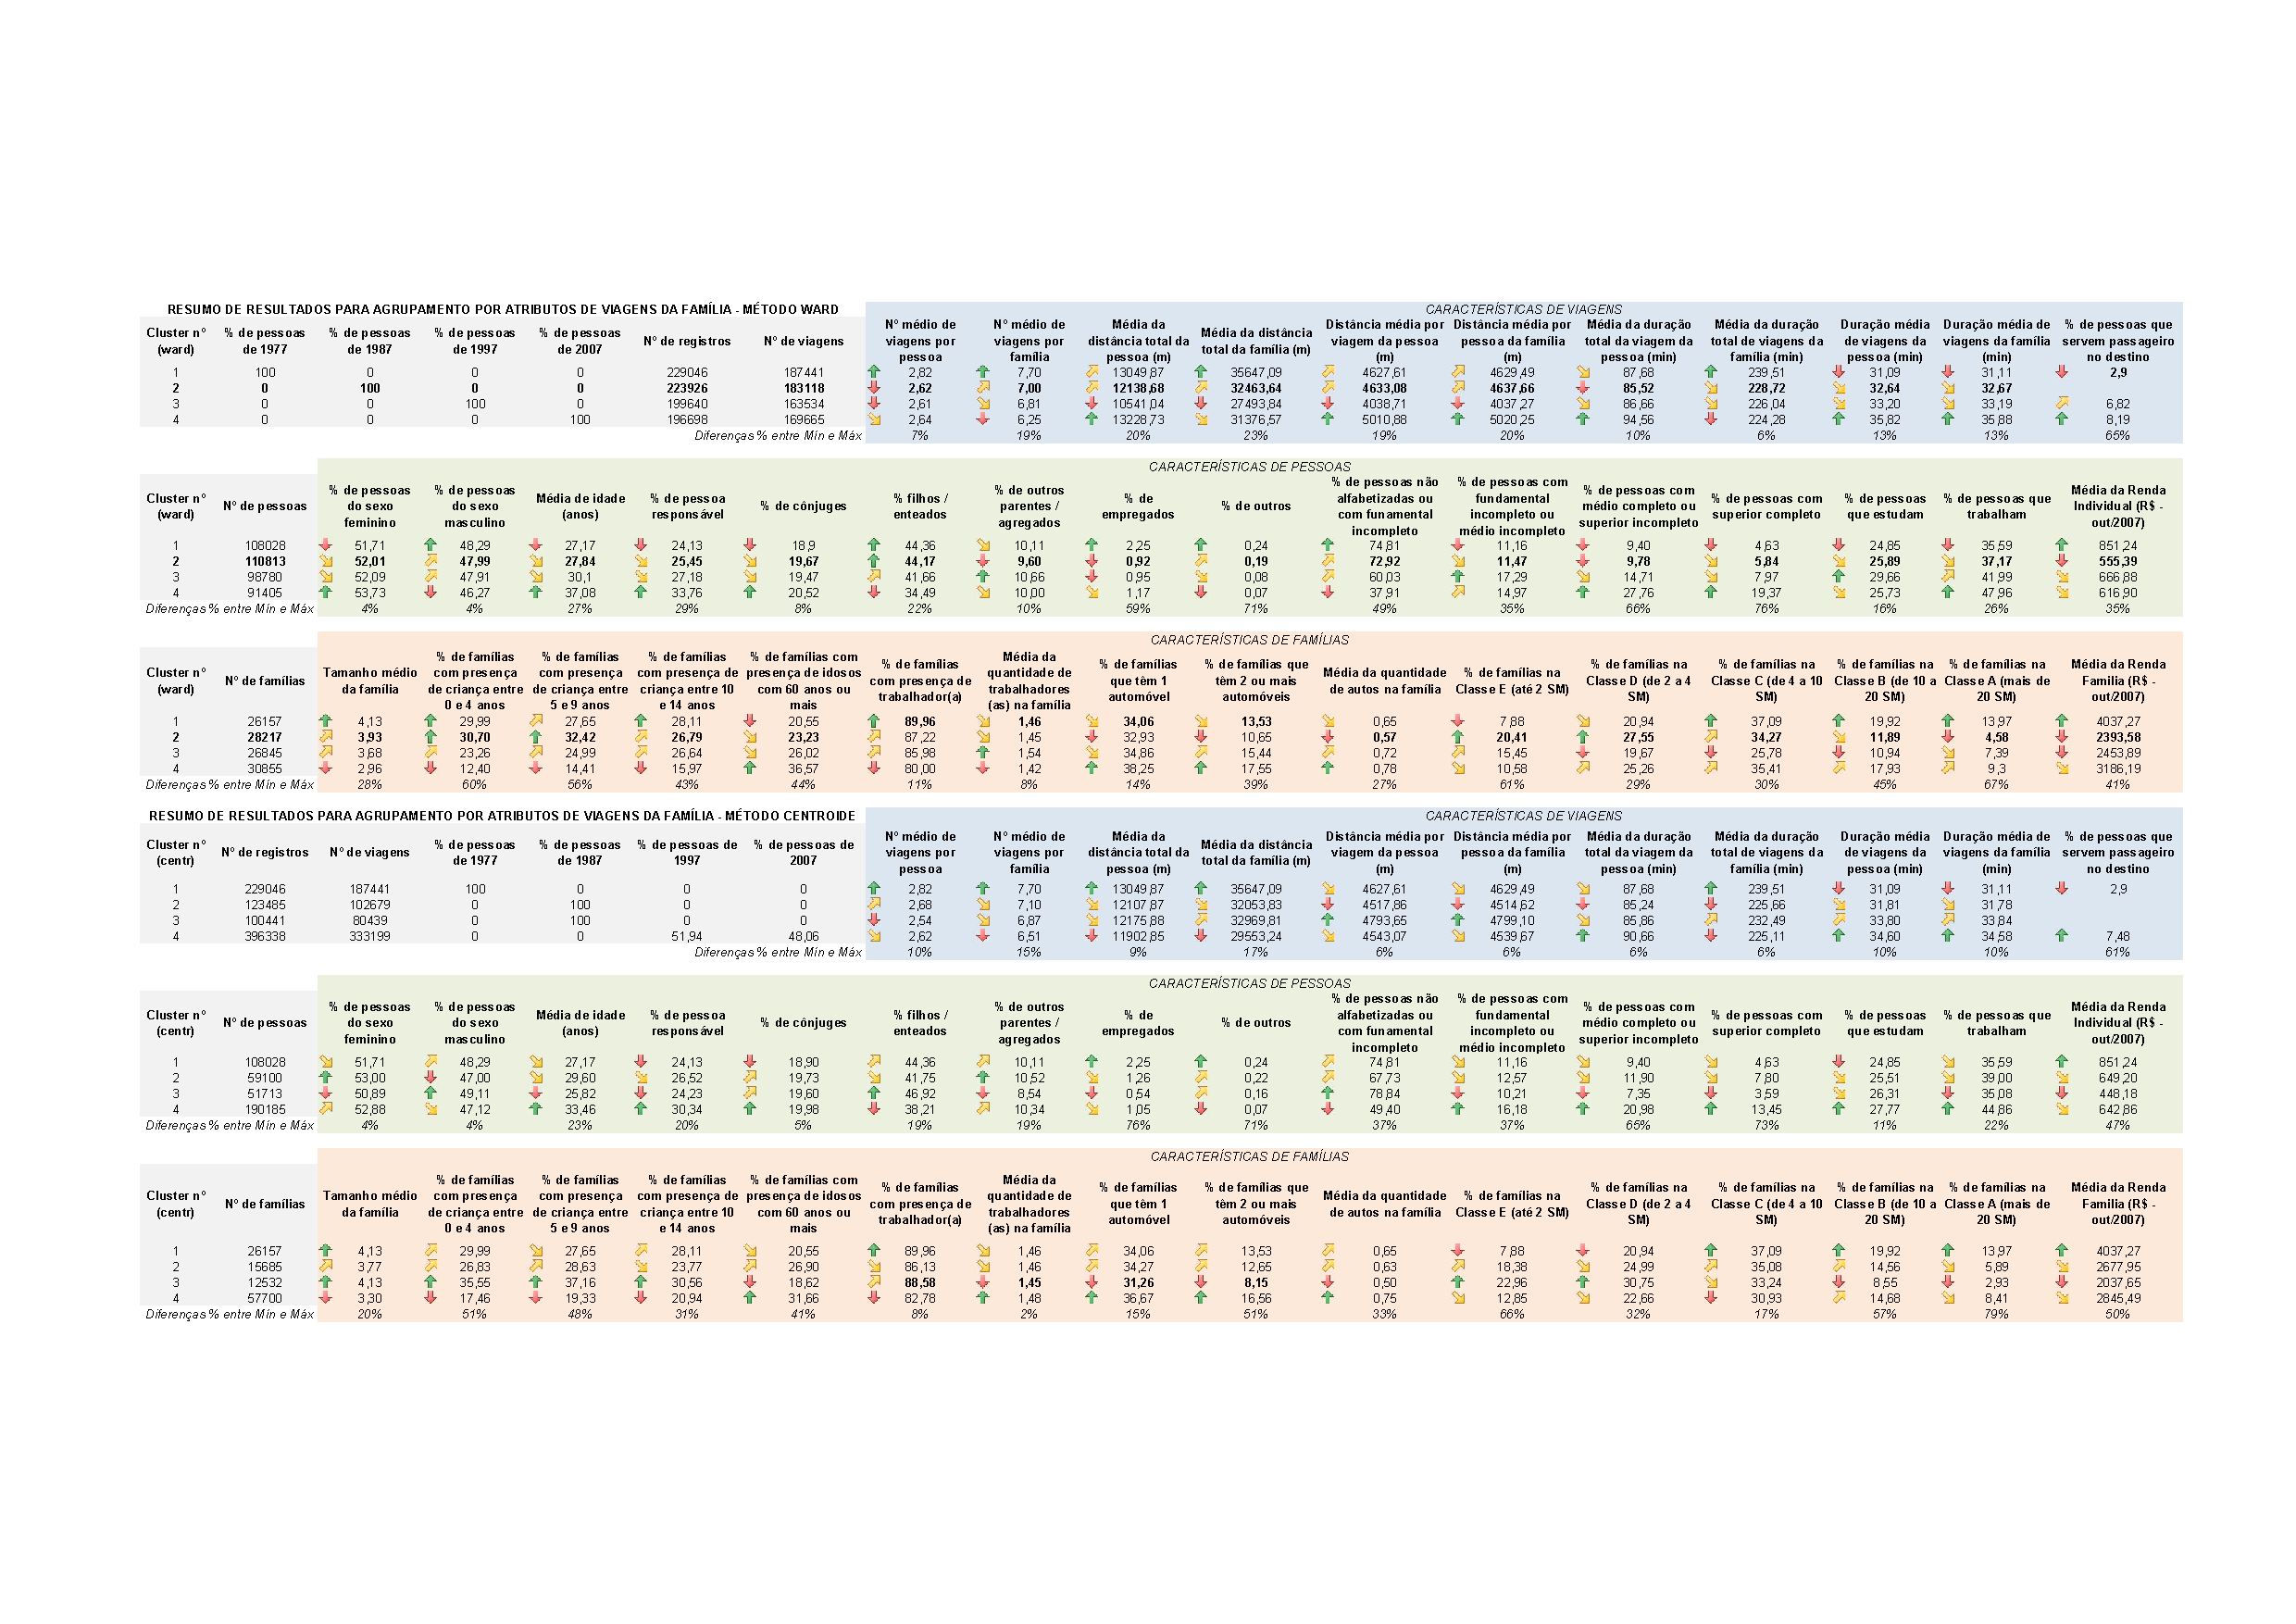
\includepdf{anexos/ResumoCluster4WardCentroide.pdf}
%% ---
%%%%%%%%%%%%%%%%%%%%%%%%%%%%%%%%%%%%%%%%%%%
%% ---
\chapter{Síntese de resultados para 4 conglomerados - segmentação por ano}\label{chap:anexo_4_clusters_fam}
%% ---
\includepdf{anexos/ResumoCluster4FAMCentroide.pdf}
\includepdf{anexos/ResumoCluster4FAMCentroide2.pdf}
%% ---
%%%%%%%%%%%%%%%%%%%%%%%%%%%%%%%%%%%%%%%%%%%
%% ---
